\documentclass[../DocumentazioneProgetto.tex]{subfiles}

\graphicspath{{../resources/2-Progetto_Completo}}

\begin{document}
	%Il progetto completo 
	\section{Il progetto completo}
	\label{sec:ProgettoCompleto}
	%Docker compose 
	\subsection{Docker compose}
	Verranno analizzate due varianti del docker compose, la prima relativa al progetto,
	la seconda relativa ad un ambiente reale.
	%Versione simulata 
	\subsubsection{Versione simulata}
	Questo è il docker compose usato nel progetto, in un ambiente reale una configurazione simile avrebbe poco senso.
	\begin{lstlisting}[language=XML, caption=Docker Compose Progetto] 
version: "3"

services:
	WebServer1:
		build: Dockerfiles/webserver/.
		image: webserver
		container_name: WS1
		networks:
			- Internal
		depends_on:
			- Syslogserver
		logging:
			driver: syslog
			options:
				syslog-address: "tcp://localhost:514"
				tag: "WS1"
		restart: unless-stopped
	WebServer2:
		build: Dockerfiles/webserver/.
		image: webserver
		container_name: WS2
		networks:
			- Internal
		depends_on:
			- Syslogserver
		logging:
			driver: syslog
			options:
				syslog-address: "tcp://localhost:514"
				tag: "WS2"
		restart: unless-stopped
	WebServer3:
		build: Dockerfiles/webserver/.
		image: webserver
		container_name: WS3
		networks:
			- Internal
		depends_on:
			- Syslogserver
		logging:
			driver: syslog
			options:
				syslog-address: "tcp://localhost:514"
				tag: "WS3"
		restart: unless-stopped
	WebServer4:
		build: Dockerfiles/webserver/.
		image: webserver
		container_name: WS4
		networks:
			- Internal
		depends_on:
			- Syslogserver
		logging:
			driver: syslog
			options:
				syslog-address: "tcp://localhost:514"
				tag: "WS4"
		restart: unless-stopped
	LoadBalancer:
		build: Dockerfiles/load-balancer/.
		image: loadbalancer
		container_name: LB
		networks:
			- Internal
			- External
		ports:
			- "80:80"
		depends_on:
			- WebServer1
			- WebServer2
			- WebServer3
			- WebServer4
			- Syslogserver
		logging:
			driver: syslog
			options:
				syslog-address: "tcp://localhost:514"
				tag: "LB"
		restart: unless-stopped
	Syslogserver:
		build: Dockerfiles/rsyslog/.
		image: syslogserver
		container_name: Syslog
		volumes:
			- "[CARTELLA LOCALE LOG]:/var/log"
		ports:
			- 514:514
			- 514:514/udp
		cap_add:
			- SYSLOG
		restart: unless-stopped

networks:
	Internal:
		internal: true
	External:\end{lstlisting}
	%Analisi Docker Compose 
	\subsubsection{Analisi Docker Compose}
	Nel file sono presenti 6 servizi di cui: 4 web server, 1 load balancer e 1 server log.\\
	In questa configurazione l'unica porta da esporre verso l'esterno è la 80 indirizzata all'ip della macchina su cui girano tutti i servizi.\\
	Verrà esposta anche la 514 ma NON è necessario esporla fuori dalla lan locale.\\
	I dettagli di configurazione dei vari servizi verranno analizzati in seguito nelle relative sezioni, si noti però
	che tutti i servizi hanno delle caratteristiche comuni:
	\begin{itemize}
		\item \textit{build}: Eventuale percorso al Dockerfile per construire l'immagine
		\item \textit{image}: Nome dell'immagine da usare O nome dell'immagine costruita tramite build
		\item \textit{container\_name}: Nome univoco nel sistema del container
		\item \textit{networks}: Lista di network a cui collegare il sistema
		\item \textit{depends\_on}: Lista di servizi da avviare prima del servizio in questione
		\item \textit{logging}
		\begin{itemize}
			\item \textit{syslog-address}: Indirizzo del server di log, in questo caso \textit{localhost} 
			\item \textit{tag}: Nome del servizio con cui identificarsi nel log server
		\end{itemize}
		\item \textit{restart}: azione da intraprendere in caso di errore o arresto anomalo
	\end{itemize}


	%Versione effettiva 
	\subsubsection{Versione effettiva} 
	Versione utile in un ambiente reale.\\
	In questo caso il load balancer e i webserver vengono eseguiti su macchine diverse.
	\begin{lstlisting}[language=XML, caption=Docker Compose Reale Load Balancer] 
version: "3"

services:
	LoadBalancer:
		build: Dockerfiles/load-balancer/.
		image: loadbalancer
		container_name: LB
		ports:
			- "80:80"
		depends_on:
			- Syslogserver
		logging:
			driver: syslog
			options:
				syslog-address: "tcp://localhost:514"
				tag: "LB"
		restart: unless-stopped
	Syslogserver:
		build: Dockerfiles/rsyslog/.
		image: syslogserver
		container_name: Syslog
		volumes:
			- "[CARTELLA LOCALE LOG]:/var/log"
		ports:
			- 514:514
			- 514:514/udp
		cap_add:
			- SYSLOG
		restart: unless-stopped\end{lstlisting}
		Nel primo file troviamo il load balancer e il server log.\\
		La porta 80 del load balancer deve essere esposta al di fuori della lan locale, la 514 del server log deve essere esposta SOLO SE le macchine su cui gireranno i webserver saranno al di fuori della rete locale.

\begin{lstlisting}[language=XML, caption=Docker Compose Reale Load Balancer] 
version: "3"

services:
	WebServer:
		build: Dockerfiles/webserver/.
		image: webserver
		container_name: WS
		depends_on:
			- Syslogserver
		logging:
			driver: syslog
			options:
				syslog-address: "tcp://[IP Syslogserver]:514"
				tag: "WS-N"
		restart: unless-stopped\end{lstlisting}
	Nel secondo file troviamo la configurazione di un webserver.\\
	Questo dockerfile verrà distribuito a tutte le macchine che dovranno ospitare un webserver.\\
	È necessario aggiornare l'indirizzo del server di log in \textit{syslog-server} con l'indirizzo della macchina su cui gira il servizio Syslogserver, è inoltre necessario inserire un id univoco nella sezione \textit{tag} del logging al fine di consentire al server log di distinguere tra le varie istanze del webserver.\\
	\textbf{Dato che non abbiamo più un network docker, è necessario esporre le porte 80 di tutti gli host alla rete interna, al fine di consentire al load balancer reindirizzare le richieste.} 

	%Screenshot funzionamento 
	\subsection{Screenshot funzionamento} 
	\begin{figure}[ht]
		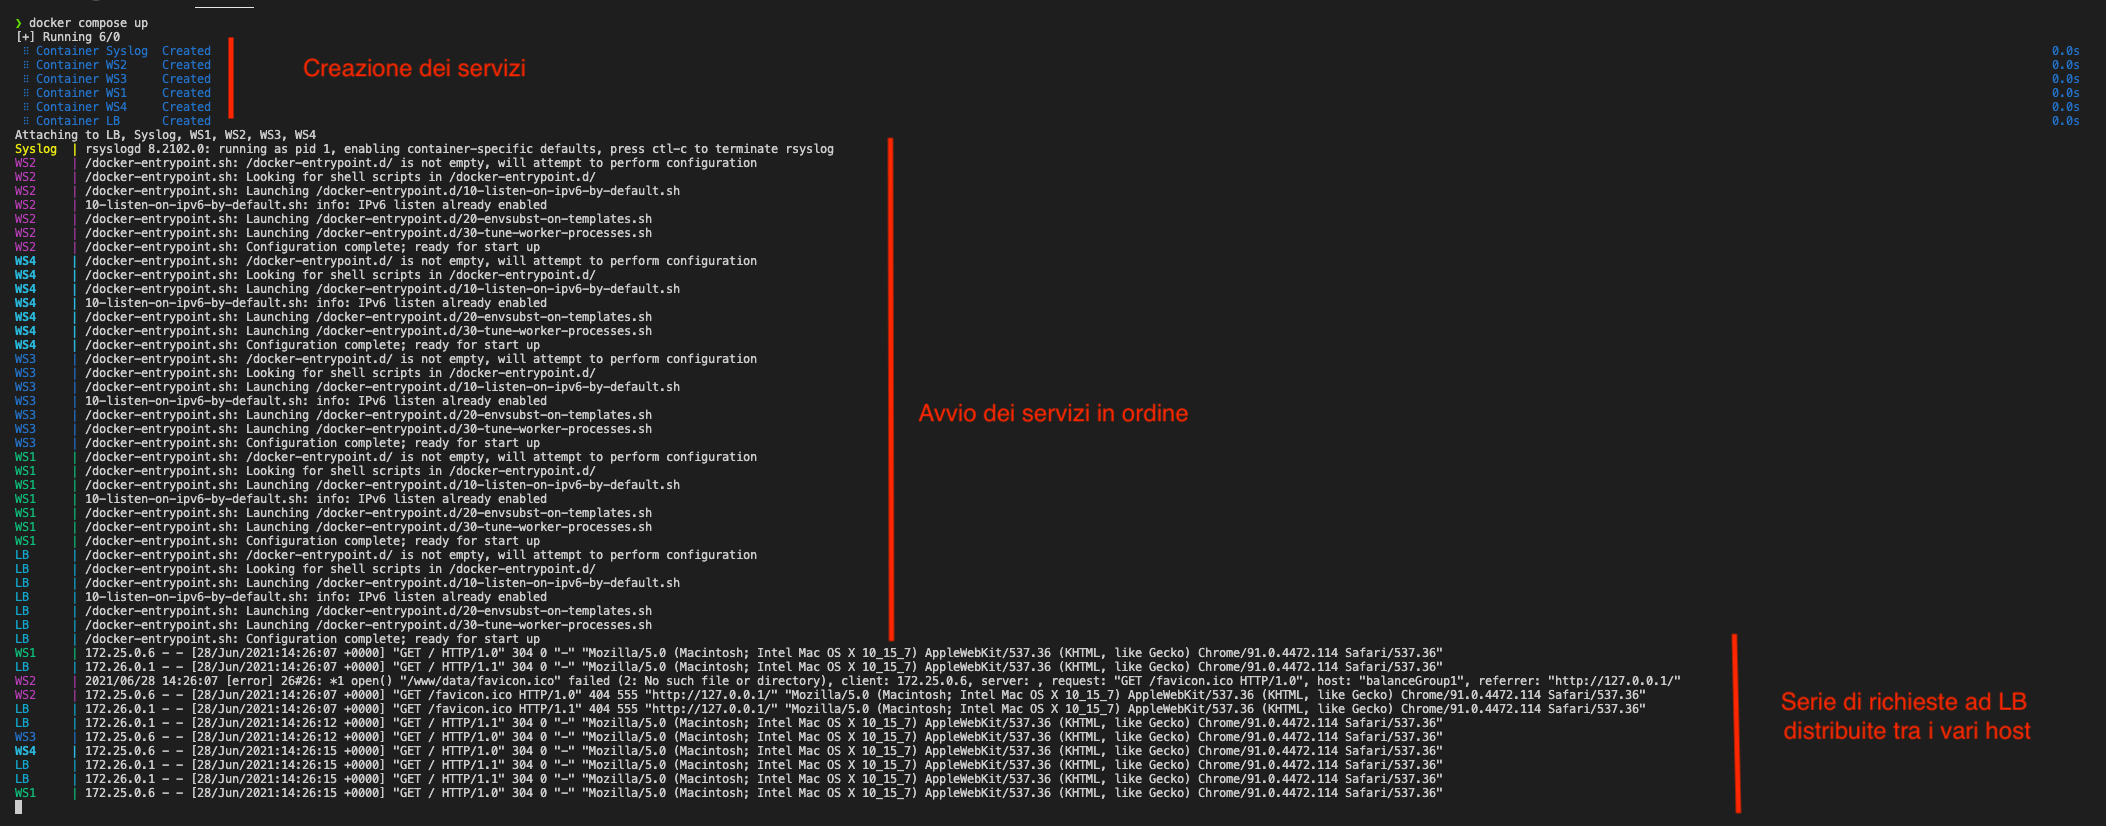
\includegraphics[width=15cm]{images/dcLog.png}
		\centering
		\caption{Log di avvio servizi e richieste distribuite}
		\label{fig:dcLog}
	\end{figure}
	Come si vede dalla \autoref{fig:dcLog}, il primo servizio avviato è il server log, seguito dai 4 webserver in parallelo e, per ultimo, dal load balancer.\\
	Una volta avviato, il load balancer risponde alle richieste dei client distribuendole tra i server definiti nel config, come visibile nelle ultime righe della \autoref{fig:dcLog}.

	\begin{figure}[ht]
		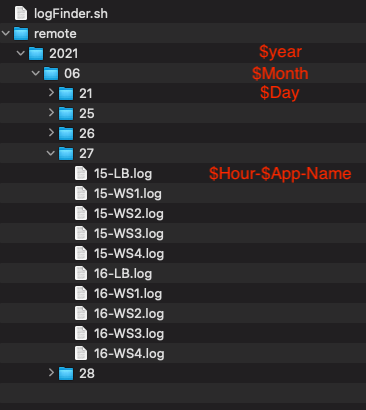
\includegraphics[width=10cm]{images/logDir.png}
		\centering
		\caption{Cartella di salvataggio server di log (\autoref{sec:Rsyslog})}
		\label{fig:logDir}
	\end{figure}
	Nella \autoref{fig:logDir} si può notare il template del server di log in azione, i file vengono suddivisi secondo il template e, come previsto, ogni ora viene generato un nuovo file di log.

	\begin{figure}[ht]
		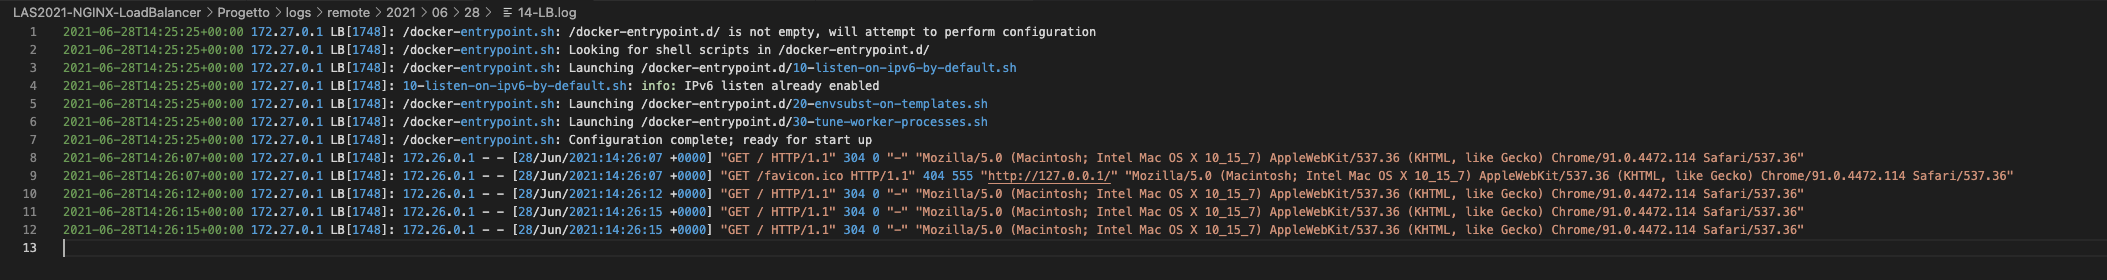
\includegraphics[width=15cm]{images/logFile.png}
		\centering
		\caption{Contenuto del file di log \textit{2021/06/28/14-LB.log}}
		\label{fig:logFile}
	\end{figure}
	La \autoref{fig:logFile} mostra il contenuto di uno dei file di log del server di log (\autoref{sec:Rsyslog}).\\
	Ogni riga contiene:
	\begin{enumerate}
		\item Un timestamp di ricezione del log
		\item Indirizzo ip del mittente
		\item Tag del servizio
		\item Pid del servizio
		\item Messaggio
	\end{enumerate}
	Come previsto i messaggi mostrati in \autoref{fig:logFile} corrispondono con i log del servizio LB visti in \autoref{fig:dcLog}.
\end{document}  